\documentclass{beamer}
\usepackage[orientation=landscape,size=a0,scale=1.0,debug]{beamerposter}
%\documentclass{article}
%\usepackage[margin=2cm]{geometry}
\usepackage{graphicx}
\usepackage{fancyvrb}
\usepackage{multicol}
\usepackage[utf8]{inputenc}
\usepackage{hyperref,tikz}
\usepackage{lipsum}
\usepackage{amsmath,amssymb}
\def\sect#1{\textbf{\color{blue} #1}}
\def\subsect#1{\underline{\color{blue} #1}}

\graphicspath{{./img//}}

\setbeamertemplate{navigation symbols}{}

\setbeamertemplate{headline}
{ 
	\vskip.5cm
	\parbox[bottom][][c]{\paperwidth} 
	{\centering
	
\includegraphics[height=6cm]{Octconf2015Logo.png}
	\hskip2cm
	
\includegraphics[height=6cm]{unilogoneu.jpg}
	\hskip2cm
	%\fbox{
	\parbox[b]{.5\paperwidth}
	{\centering
	  \mbox{}\\
	 {\color{structure.fg}\Huge\inserttitle{}}\\[4ex]
	 {\Large \insertauthor{}}\\[10ex]
	  \mbox{}
	} % end parbox
	%} % end fbox
	\hskip2cm
	
\includegraphics[height=6cm]{Gnu-octave-logo.png}
	\hskip2cm
	
\includegraphics[height=6cm]{tudarmstadt.png}
	} % end parbox
} % end setbeamertemplate headline

\title{Examples for teaching mathematical programming 
       using \emph{Octave}}
\author{Alf Gerisch (TU Darmstadt) and 
   Markus Köbis (Uni Halle) and Helmut Podhaisky (Uni Halle)}
%\date{22 September 2015}
\date{} % Damit wird leider trotzdem Platz reserviert...
%\maketitle

\begin{document}

\begin{frame}[t]{}
\begin{multicols}{5}
% %%%%%%%%%%%%%%%%%%%%%%%%%%%%%%%%%%%%%%%%%%%%%%%%%%%%%%%%%%%%%%%%%%%%%%%%%%%%%%
% ABSTRACT %%%%%%%%%%%%%%%%%%%%%%%%%%%%%%%%%%%%%%%%%%%%%%%%%%%%%%%%%%%%%%%%%%%%%
% %%%%%%%%%%%%%%%%%%%%%%%%%%%%%%%%%%%%%%%%%%%%%%%%%%%%%%%%%%%%%%%%%%%%%%%%%%%%%%
\sect{Abstract}

We believe that mathematical programming can be taught using surprising and
nontrivial examples. Short programs shall visualise an idea.  To learn how to
write correct code is easier with discrete problems where rounding errors
cannot conceal bugs.  The lack of certain data structures (lists with
$\mathcal{O}(1)$ append, queues, \dots) in Octave leads to uglier code or wrong
asymptotic complexity for some problems (shortest paths, minimal spanning
trees, \dots). Visit \url{https://github.com/hpodhaisky/OctConf} for download.

\medskip 

% %%%%%%%%%%%%%%%%%%%%%%%%%%%%%%%%%%%%%%%%%%%%%%%%%%%%%%%%%%%%%%%%%%%%%%%%%%%%%%
% CELLULAR AUTOMATONS %%%%%%%%%%%%%%%%%%%%%%%%%%%%%%%%%%%%%%%%%%%%%%%%%%%%%%%%%%
% %%%%%%%%%%%%%%%%%%%%%%%%%%%%%%%%%%%%%%%%%%%%%%%%%%%%%%%%%%%%%%%%%%%%%%%%%%%%%%
\sect{Cellular Automatons}

\begin{figure}
\VerbatimInput[frame=single, label=automaton.m, fontsize=\small]{automaton.m}
\caption{The 256 different functions $f_r\colon\{0,1\}^3\to\{0,1\}$, $f_r\colon (x^{i}_{j-1},x^{i}_j,x^{i}_{j+1})\mapsto x^{i+1}_j$
are encoded with one value $r\in \{0,\dots,255\}$.
The evolution of the one-dimensional system over time is from top to bottom. 
The graphics with \texttt{spy} is slow.}
\end{figure}

\begin{figure}
\begin{tabular}{ccc}
rule 30 & rule 90 & rule 110 \\
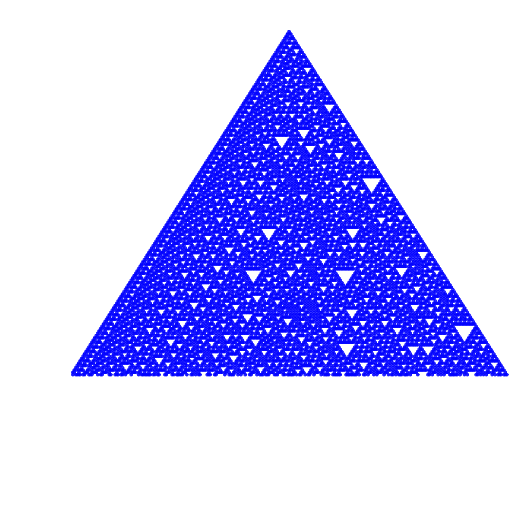
\includegraphics[width=0.3\hsize]{r30.png} & 
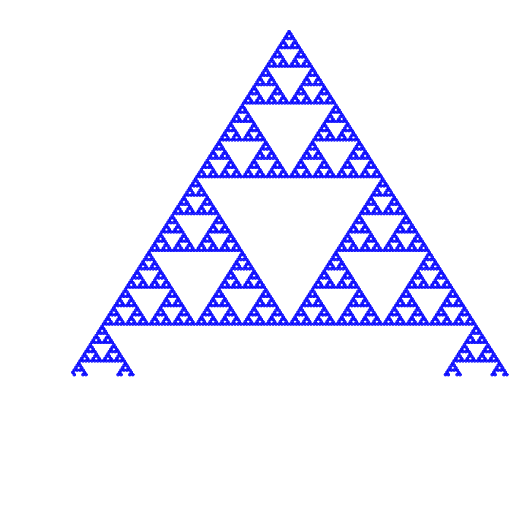
\includegraphics[width=0.3\hsize]{r90.png} & 
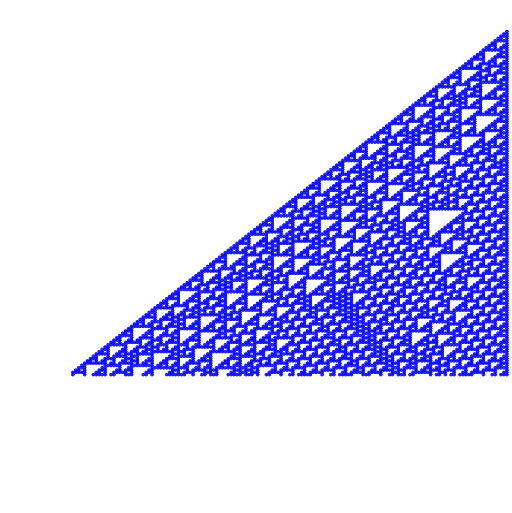
\includegraphics[width=0.3\hsize]{r110.png} 
\end{tabular}
\caption{Generated with \texttt{automaton.m}. There is chaos, structure and even
universal computation \cite{rule110}.}
\end{figure}

\begin{figure}
\VerbatimInput[frame=single, label=cells.m, fontsize=\small]{cells.m}
\caption{A cell in state $z$ is eaten by a neighbouring cell in state $z+1$.
A level of indirection makes the computation concise as well as fast. }
\end{figure}

\begin{figure}
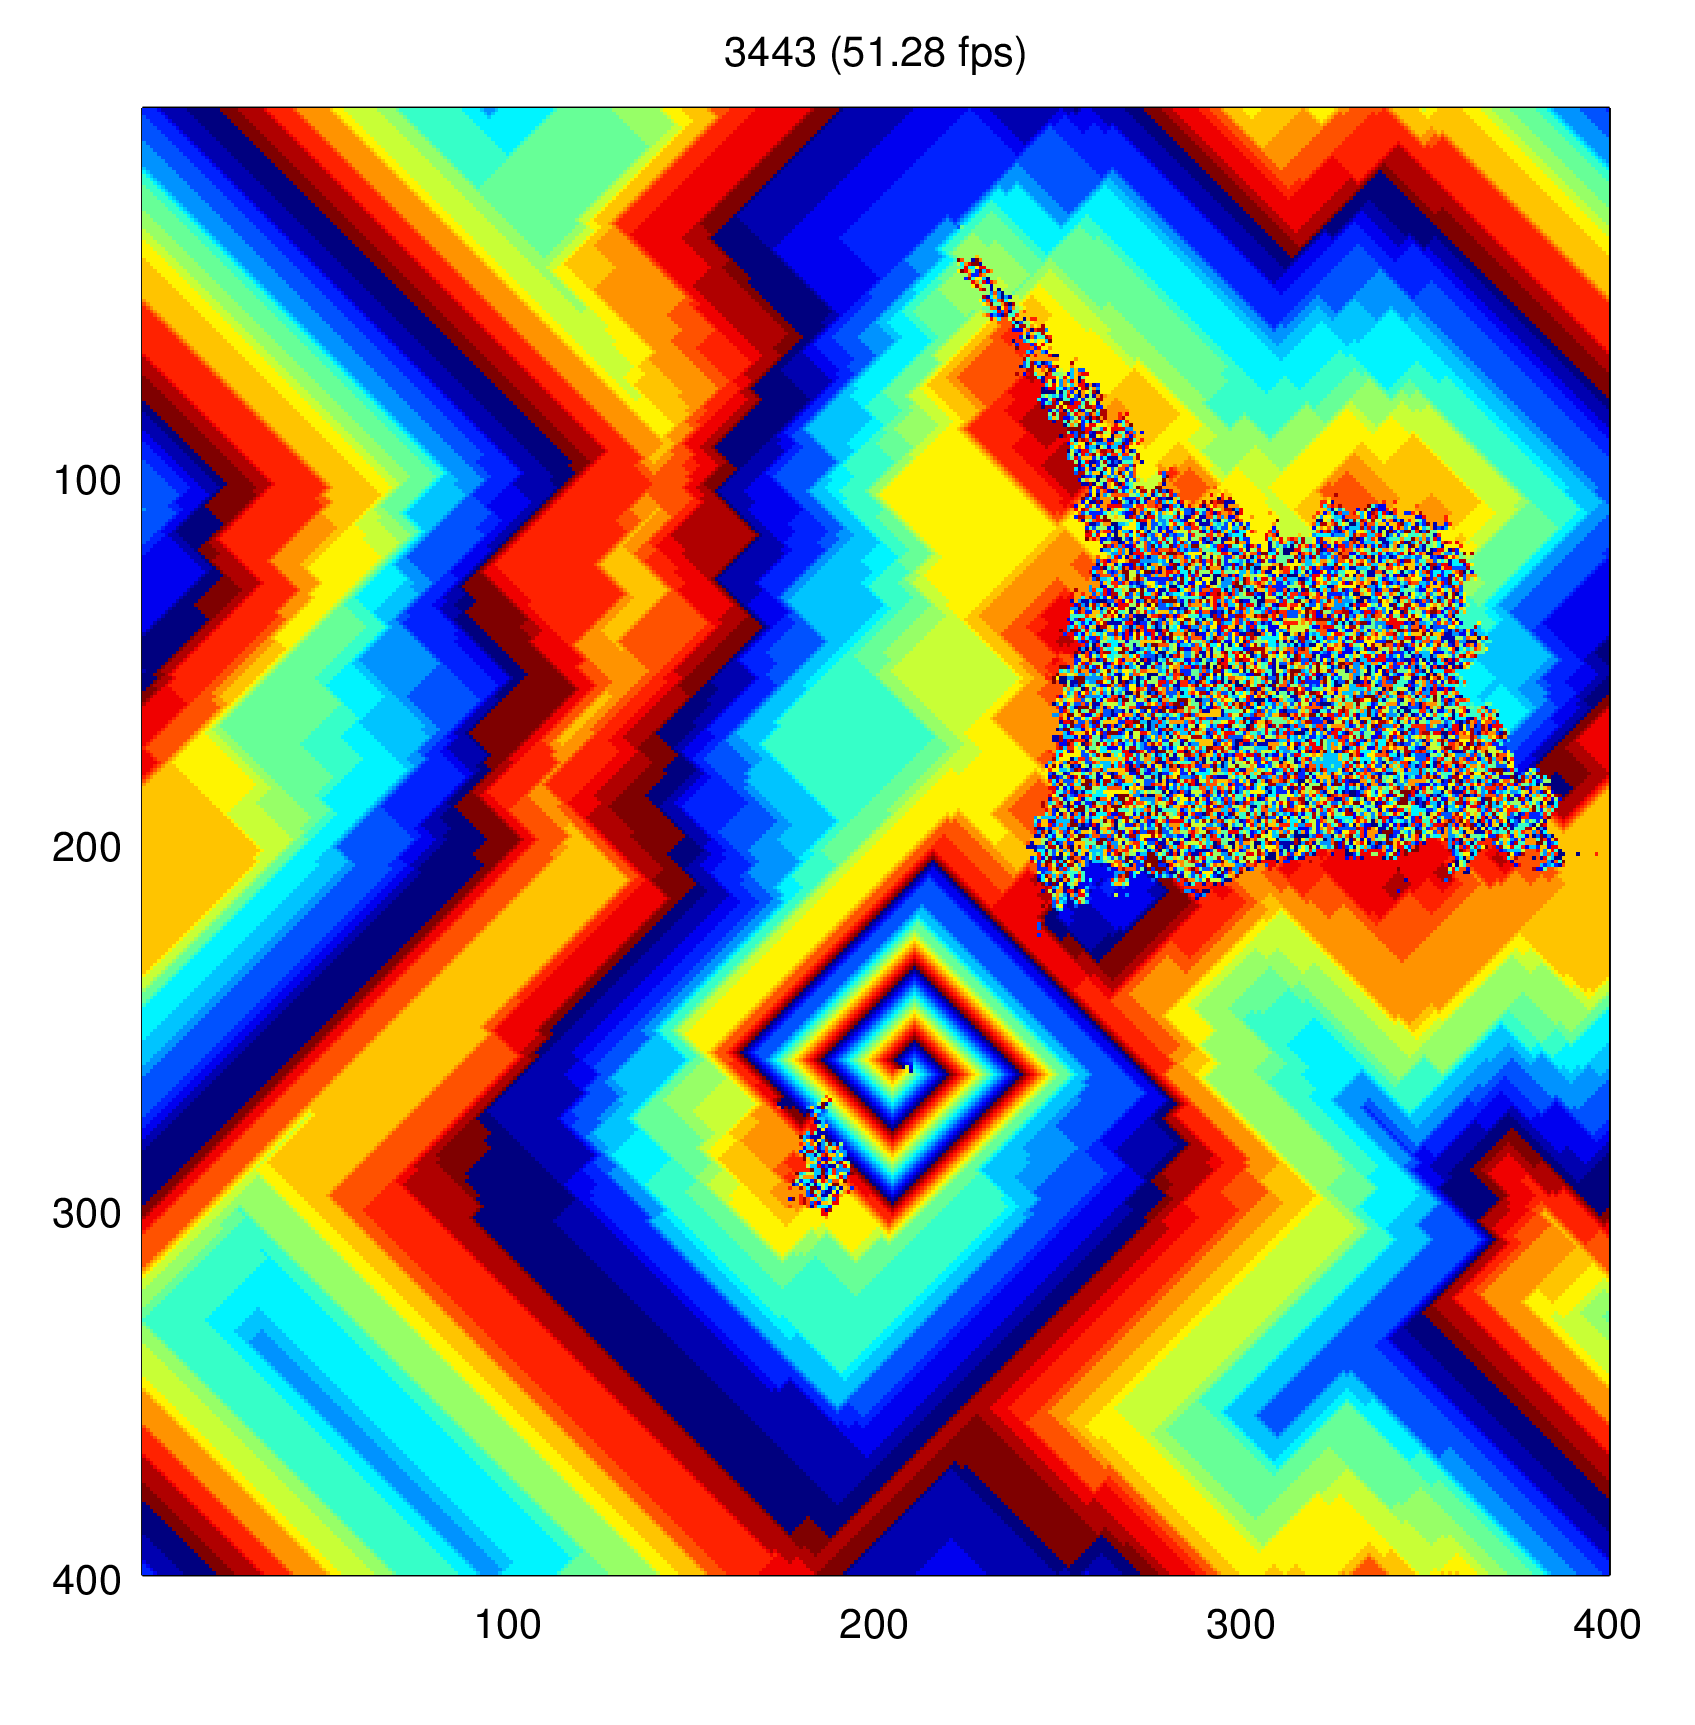
\includegraphics[width=0.75\hsize]{cells.png}
\caption{Life in a cyclic world \cite{cca}, generated with \texttt{cells.m}.
This is a snapshot of a movie in which rotating spirals arise out of chaos.
}
\end{figure}

\columnbreak

% %%%%%%%%%%%%%%%%%%%%%%%%%%%%%%%%%%%%%%%%%%%%%%%%%%%%%%%%%%%%%%%%%%%%%%%%%%%%%%
% REACTION DIFFUSION EQUATIONS %%%%%%%%%%%%%%%%%%%%%%%%%%%%%%%%%%%%%%%%%%%%%%%%%
% %%%%%%%%%%%%%%%%%%%%%%%%%%%%%%%%%%%%%%%%%%%%%%%%%%%%%%%%%%%%%%%%%%%%%%%%%%%%%%
\sect{Reaction diffusion equations}

\begin{figure}
\VerbatimInput[frame=single, label=grayscott.m, fontsize=\small]{grayscott.m}
\caption{Solving $u_t = D_u \Delta u - uv^2 + F(1-u), v_t = D_v \Delta v + uv^2 - (F+k) v$
with periodic boundary conditions using central differences for the
Laplacians and the explicit Euler method 
for integration.}

\end{figure}
\begin{figure}
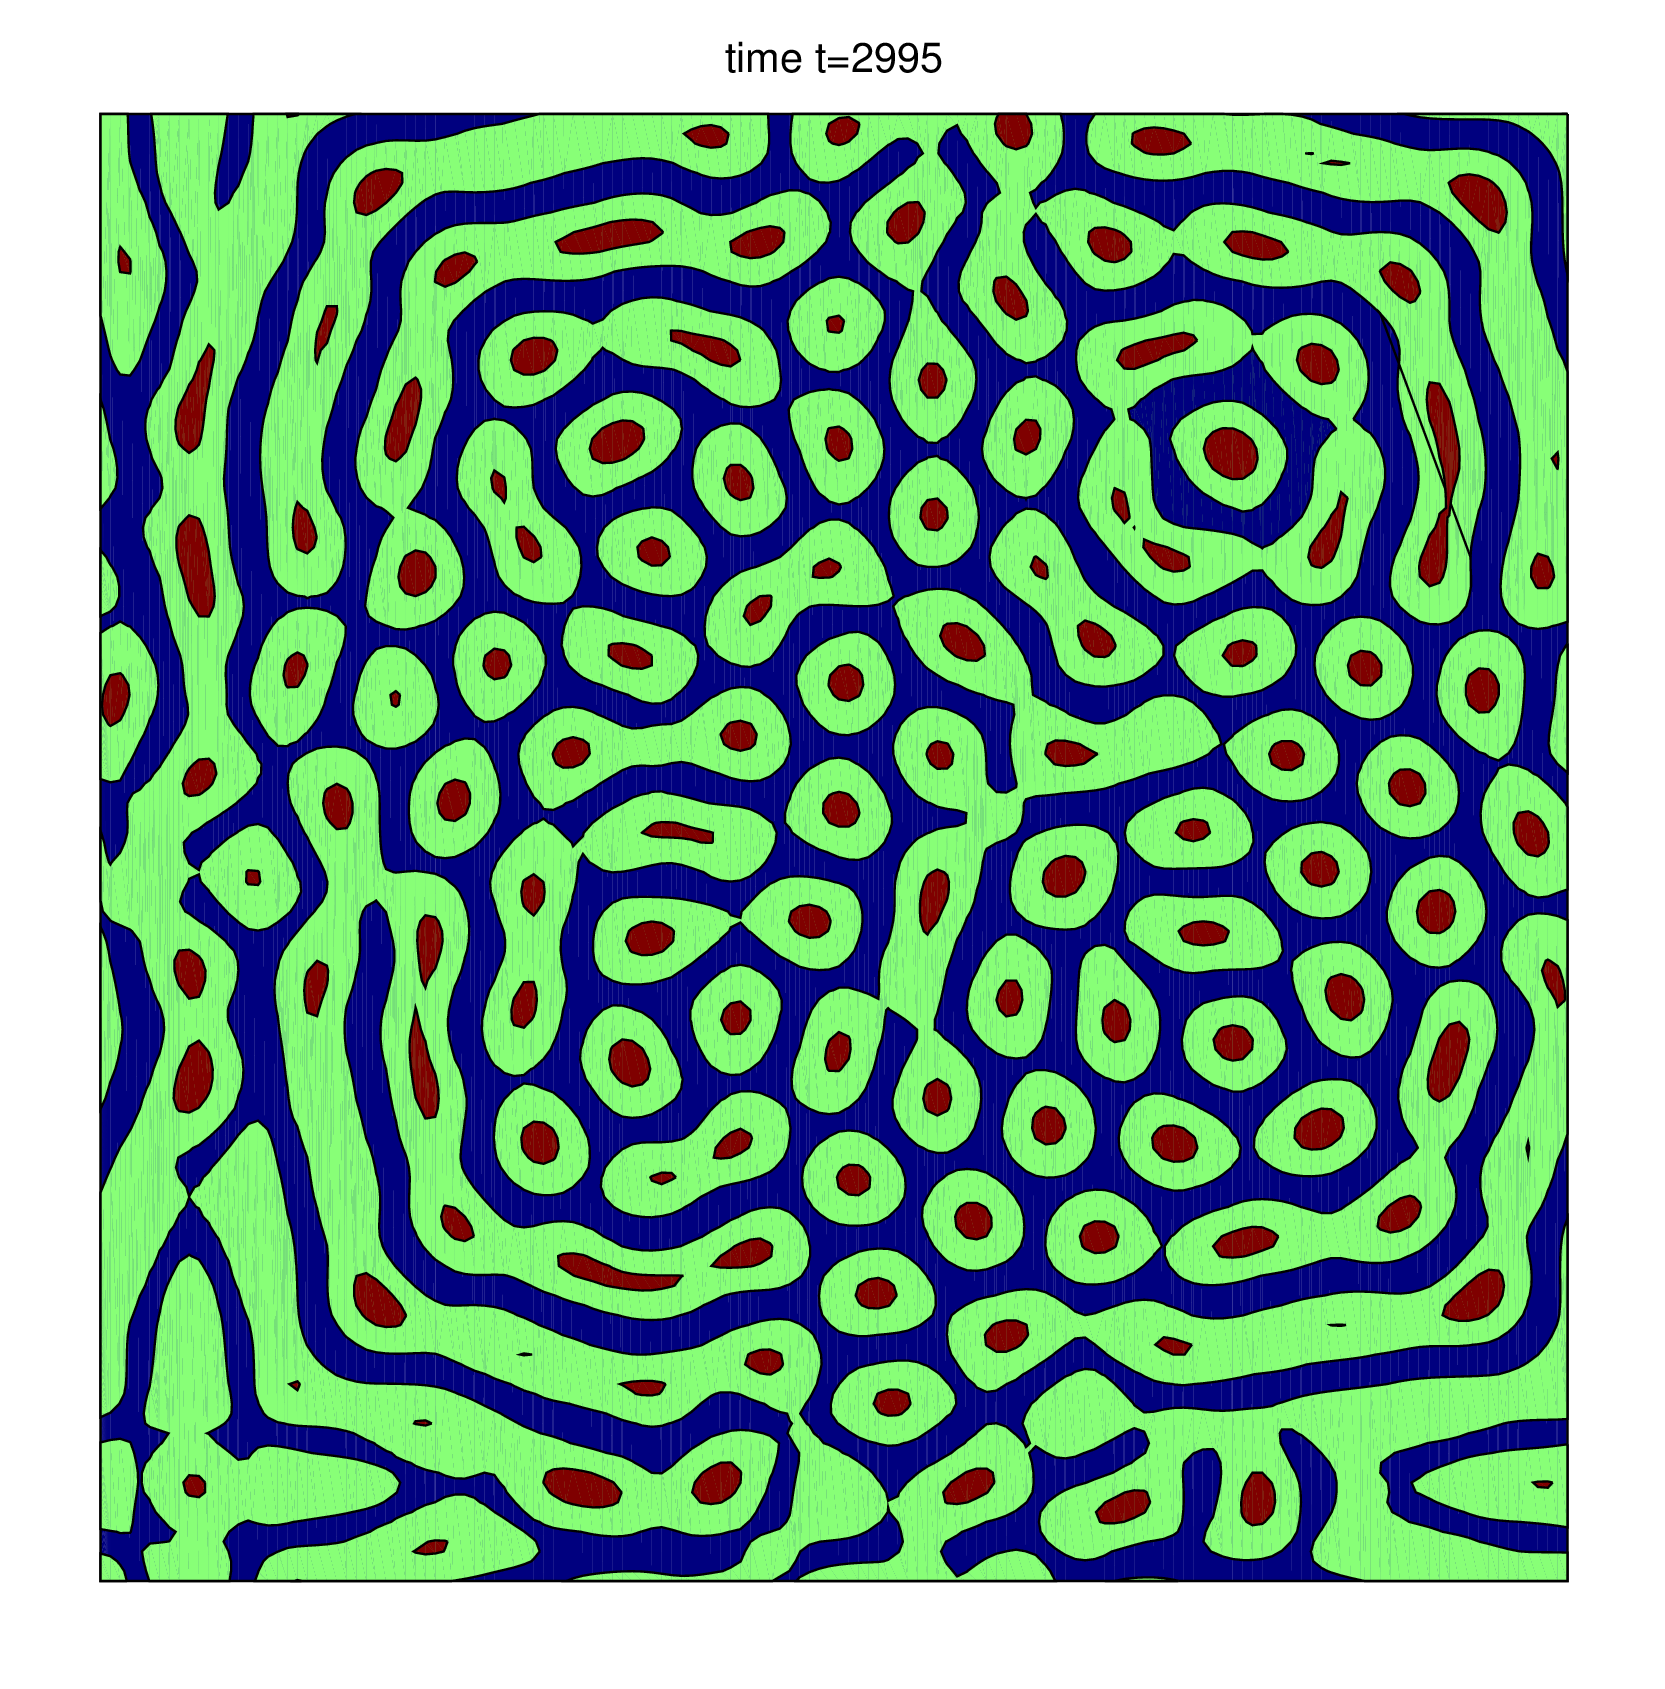
\includegraphics[width=0.75\hsize]{grayscott.png}
\caption{Self-organization in the Gray-Scott reaction-diffusion system~\cite{pearson}, generated with \texttt{grayscott.m}.}
\end{figure}

\medskip

% %%%%%%%%%%%%%%%%%%%%%%%%%%%%%%%%%%%%%%%%%%%%%%%%%%%%%%%%%%%%%%%%%%%%%%%%%%%%%%
% LINDENMAYERS L-SYSTEMS %%%%%%%%%%%%%%%%%%%%%%%%%%%%%%%%%%%%%%%%%%%%%%%%%%%%%%%
% %%%%%%%%%%%%%%%%%%%%%%%%%%%%%%%%%%%%%%%%%%%%%%%%%%%%%%%%%%%%%%%%%%%%%%%%%%%%%%
\sect{Lindenmayer's L-systems}

\begin{figure}
\VerbatimInput[frame=single, fontsize=\small, label=lsystem.m]{lsystem.m}
\caption{Adapted from \cite{matlabguide}. We use complex multiplication for 
rotation and recursion to avoid maintaining a stack of coordinates. 
Line segments are separated by NaNs for efficient plotting.}
\end{figure}

\begin{figure}
\begin{tabular}{cccc}
\footnotesize\texttt{
F[+F][-F][++F][--F]} & 
\footnotesize\texttt{
F[+F]F[-F][F]} &
\footnotesize\texttt{
FF-[-F+F+F]+[+F-F-F]} \\
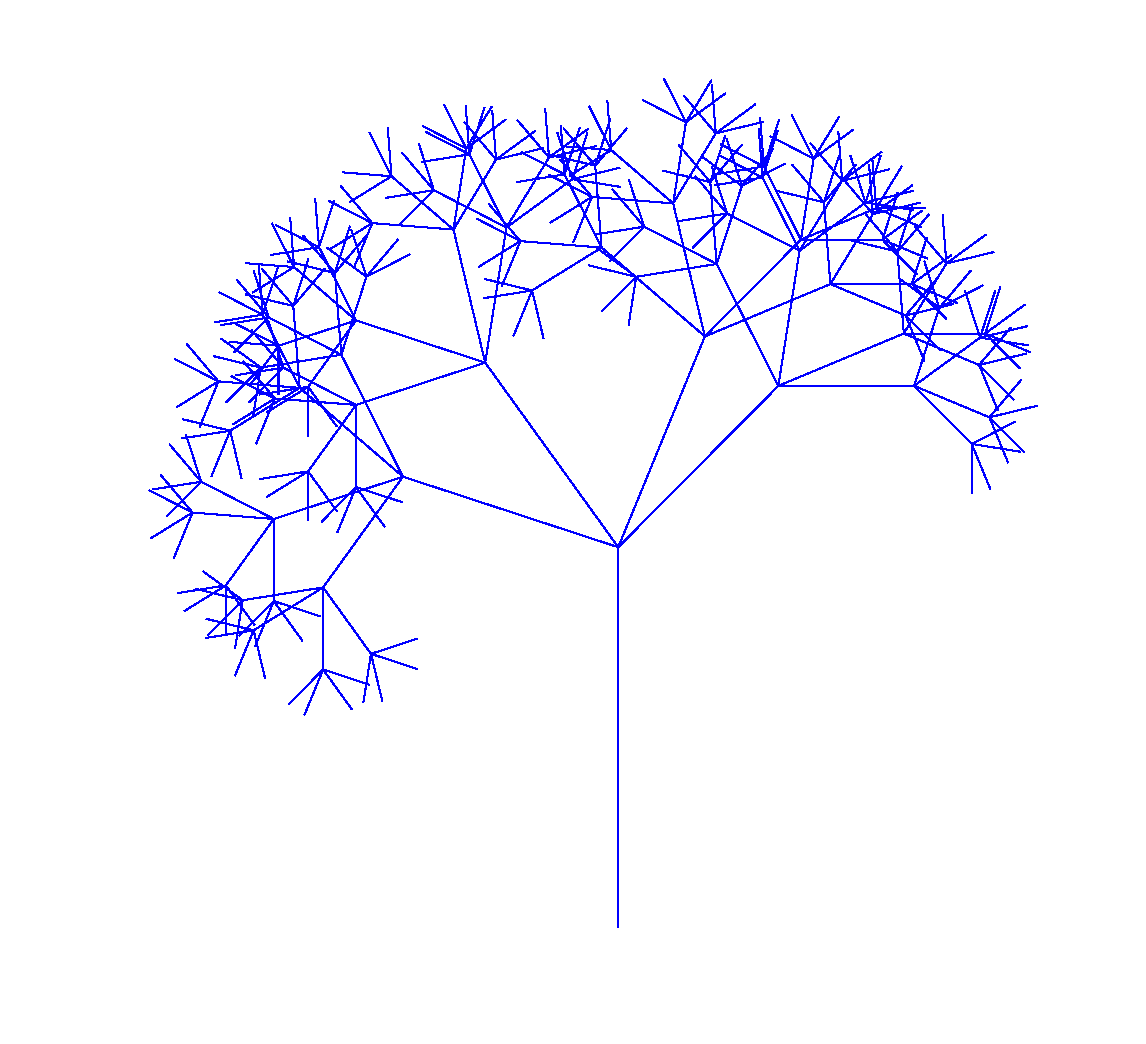
\includegraphics[width=0.3\hsize]{lsystem1} & 
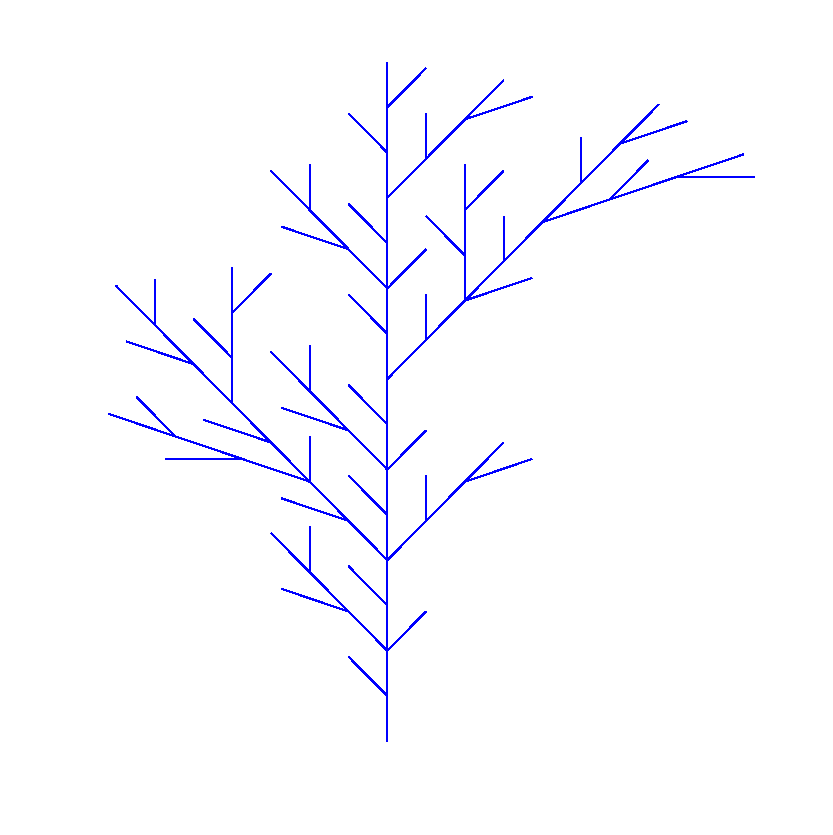
\includegraphics[width=0.3\hsize]{lsystem2} & 
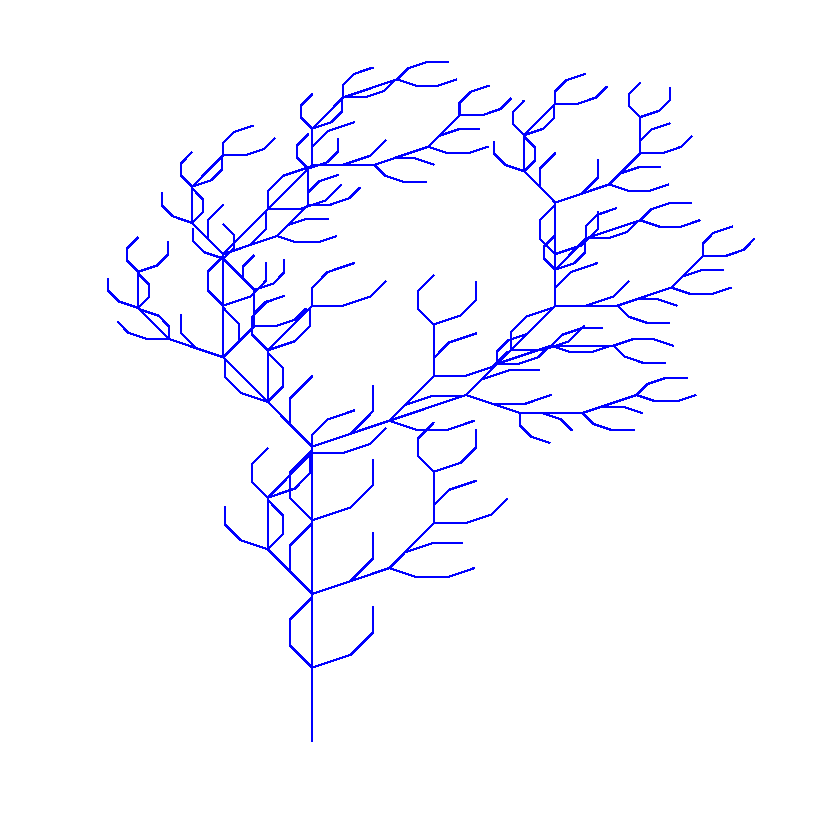
\includegraphics[width=0.3\hsize]{lsystem3} & 
\end{tabular}
\caption{Plants as generated with \texttt{lsystem.m}, cf. \cite{matlabguide}.}
\end{figure}
\medskip

% %%%%%%%%%%%%%%%%%%%%%%%%%%%%%%%%%%%%%%%%%%%%%%%%%%%%%%%%%%%%%%%%%%%%%%%%%%%%%%
% SOMA CUBE %%%%%%%%%%%%%%%%%%%%%%%%%%%%%%%%%%%%%%%%%%%%%%%%%%%%%%%%%%%%%%%%%%%%
% %%%%%%%%%%%%%%%%%%%%%%%%%%%%%%%%%%%%%%%%%%%%%%%%%%%%%%%%%%%%%%%%%%%%%%%%%%%%%%
\sect{Soma cube}

\begin{figure}
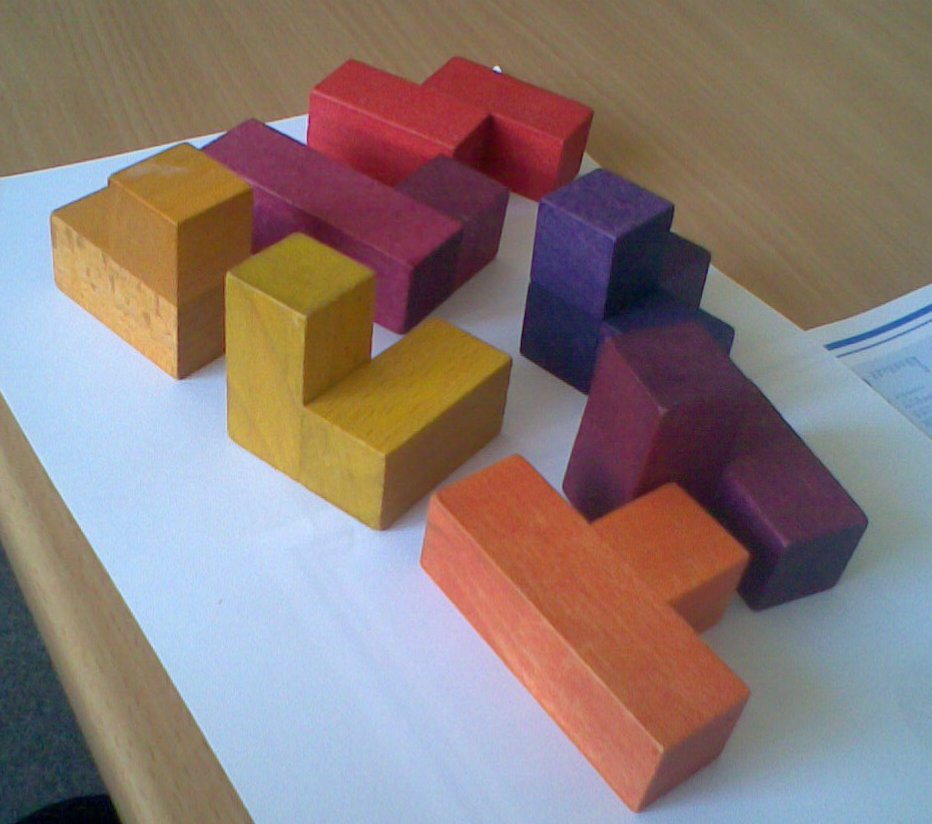
\includegraphics[width=0.3\hsize]{Soma.jpg} \hfill
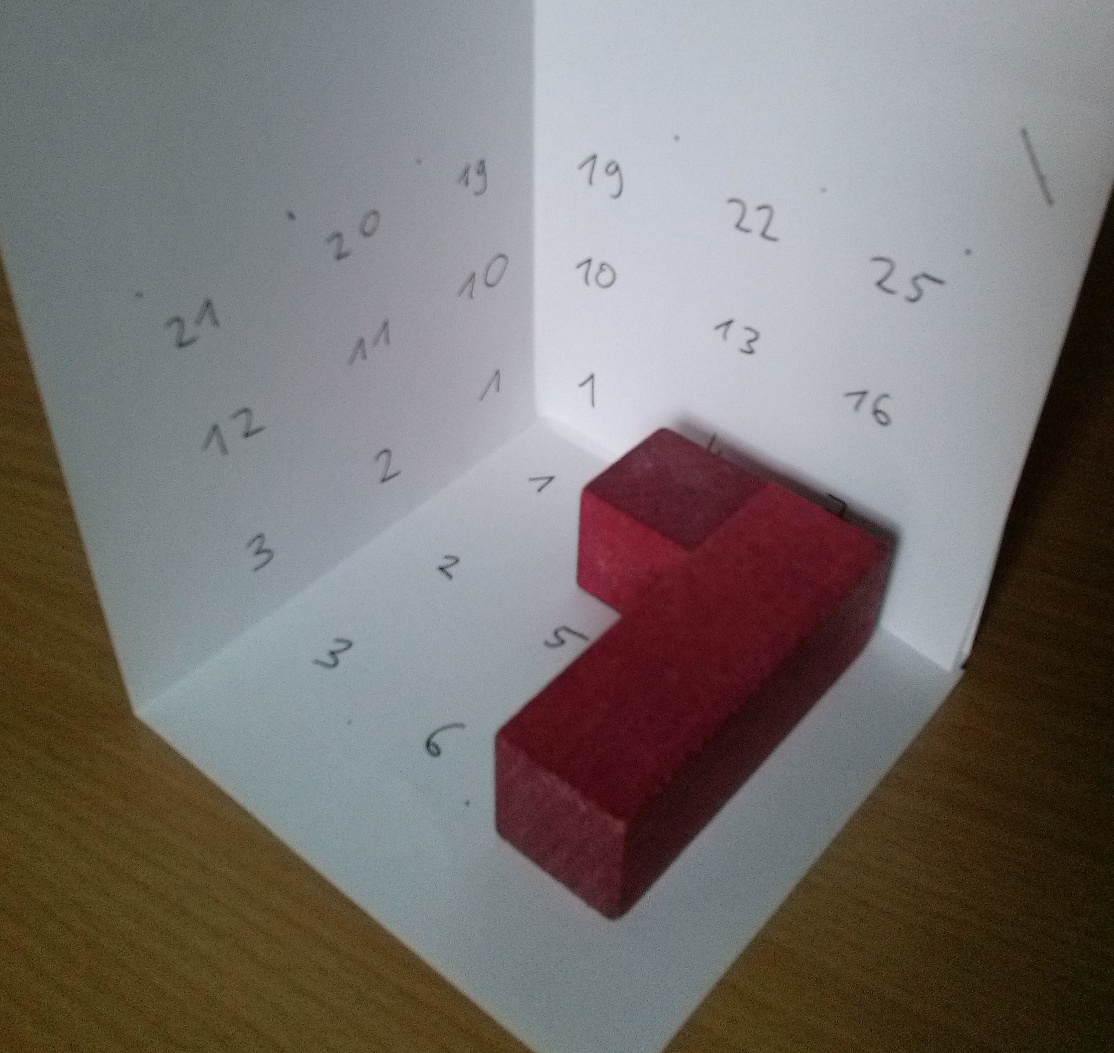
\includegraphics[width=0.3\hsize]{Soma1.jpg} \hfill
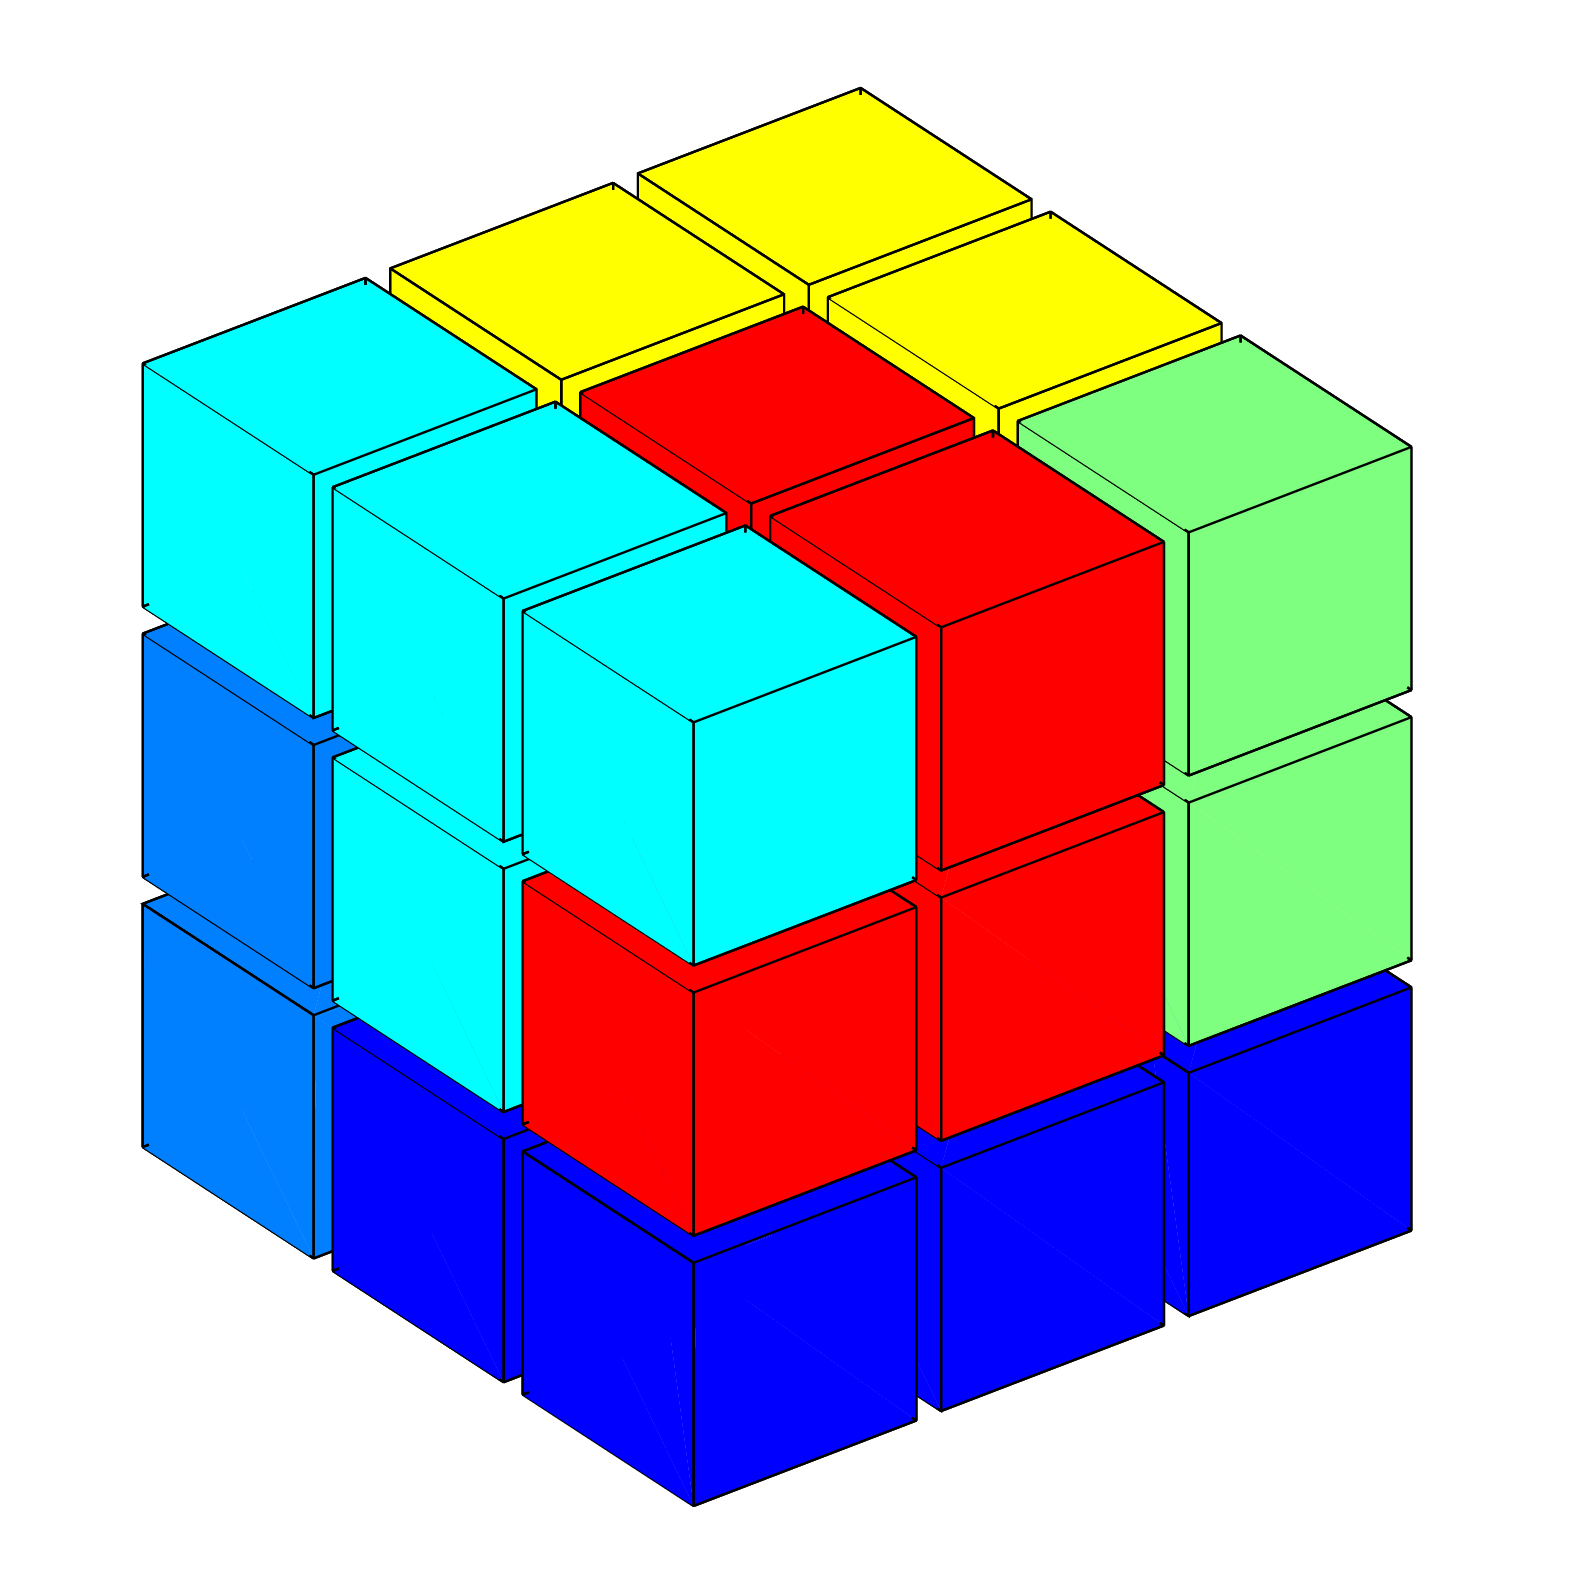
\includegraphics[width=0.3\hsize]{soma.png}
\caption{
Soma cube. Filling the space with properly aligned pieces is an instance of a
set-cover problem: Given a set of subsets, $s_i\subset \Omega$, find selection
$x$ such that $\mathop{\dot{\cup}}\limits_{i\in x} s_i=\Omega$.  There are 480
distinct ways to assemble the cube \cite{soma} and \texttt{soma.m} computes
them in a few seconds.}
\end{figure}


\begin{figure}
\VerbatimInput[frame=single, label=soma.m, fontsize=\small]{soma.m}
\caption{
We calculate valid placements for each piece in an empty cube (using rotations
\cite{oct} and shift, whereas the L shaped piece No. 1 is not rotated to fix
the rotational symmetry). The physical space $3\times 3\times 3$ is extended by
seven components to mark the number of the piece, leading
to $A x = b$ with $A\in\{0,1\}^{34\times 550}$, $x\in\{0,1\}^{550}$ and
$b=[1,\dots,1]^\top$ which is solved by backtracking.}
\end{figure}

\begin{figure}
\VerbatimInput[frame=single, fontsize=\small, label=somadraw.m]{somadraw.m}
\caption{We're drawing complete and incomplete solutions during the calculation.}
\end{figure}

\medskip


% %%%%%%%%%%%%%%%%%%%%%%%%%%%%%%%%%%%%%%%%%%%%%%%%%%%%%%%%%%%%%%%%%%%%%%%%%%%%%%
% SINGULAR VALUE DECOMPOSITION %%%%%%%%%%%%%%%%%%%%%%%%%%%%%%%%%%%%%%%%%%%%%%%%%
% %%%%%%%%%%%%%%%%%%%%%%%%%%%%%%%%%%%%%%%%%%%%%%%%%%%%%%%%%%%%%%%%%%%%%%%%%%%%%%
\sect{Singular value decomposition}

\subsect{Data compression}

\begin{figure}%
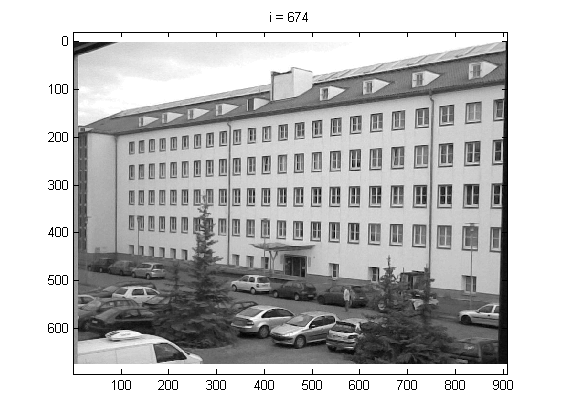
\includegraphics[width=.24\columnwidth]{VSP5full}\mbox{}%
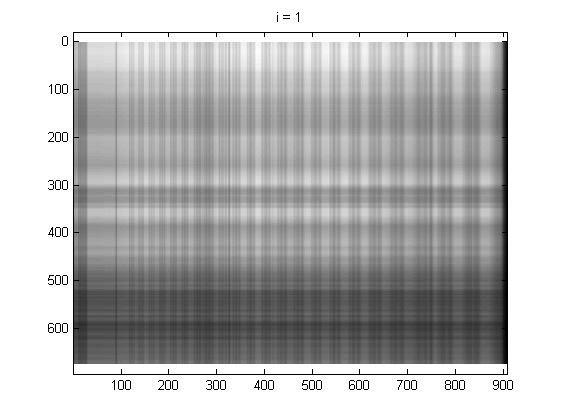
\includegraphics[width=.24\columnwidth]{VSP51}\mbox{}%
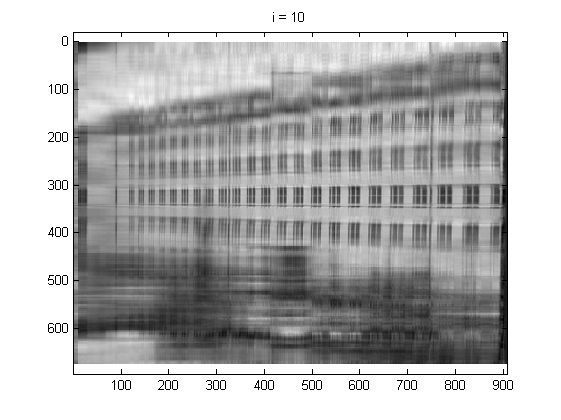
\includegraphics[width=.24\columnwidth]{VSP510}\mbox{}%
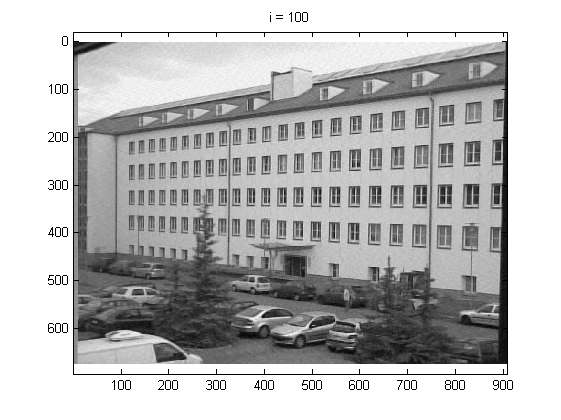
\includegraphics[width=.24\columnwidth]{VSP5100}\mbox{}%
\caption{Decomposition of a given bitmap and its reconstructions using
         $1$, $10$ and $100$ modes using \texttt{datacompression.m}
				}%
\end{figure}

\begin{figure}
\VerbatimInput[frame=single, label=datacompression.m, fontsize=\small]{markus.m}
\caption{We handle the grayscale image as matrix input and reconstruct it step-by-step
         using its principal components aquired by \emph{Octave}'s \texttt{svd.m} routine.
        }
\end{figure}

\subsect{Face recognition}

\begin{figure}
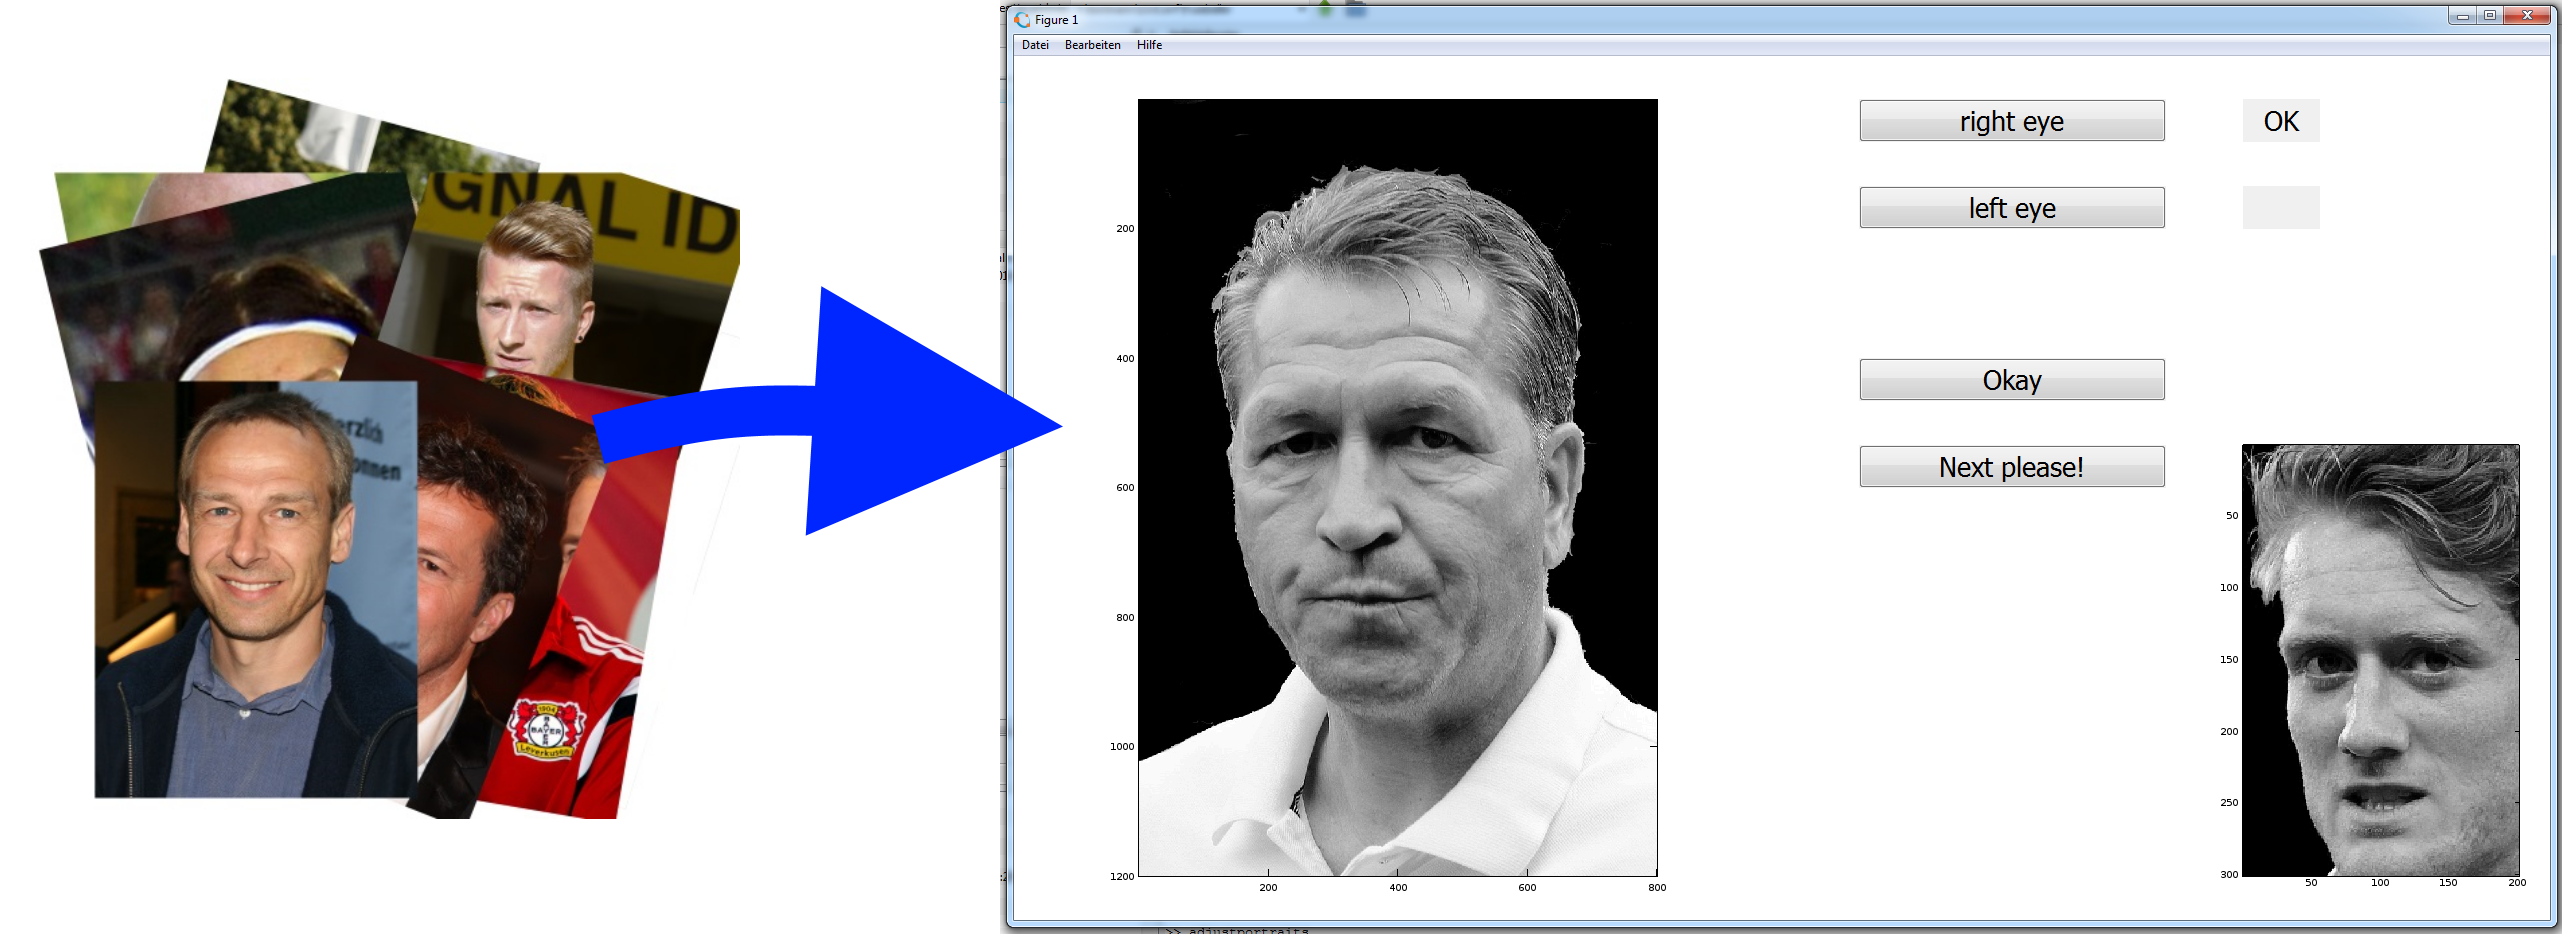
\includegraphics[width=0.95\hsize]{GUIalles.png} %\hfill
\caption{Adjusting the face orientation and eye position using graphical user interface}
\end{figure}

\begin{figure}
\VerbatimInput[frame=single,label=adjustportrait.m, fontsize=\small,lastline=22]{adjustportrait.m}
\caption{Building the graphical user interface with \texttt{uicontrol.m}, code snippet
        }
\end{figure}


\begin{figure}
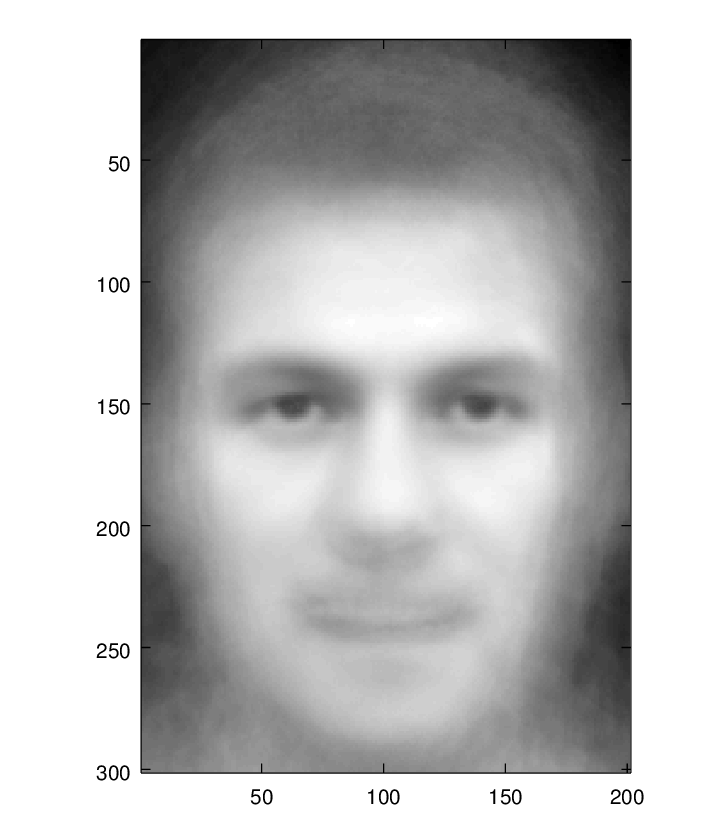
\includegraphics[height=0.53\hsize]{avrgface.png} \hfill
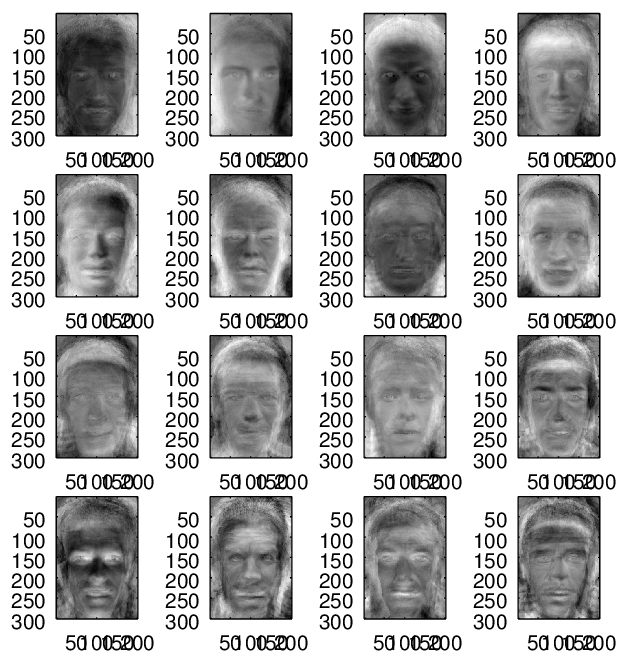
\includegraphics[height=0.53\hsize]{eigenfaces.png}
\caption{Calculating the average face from the portraits in the database and `eigenfaces'}
\end{figure}

\begin{figure}
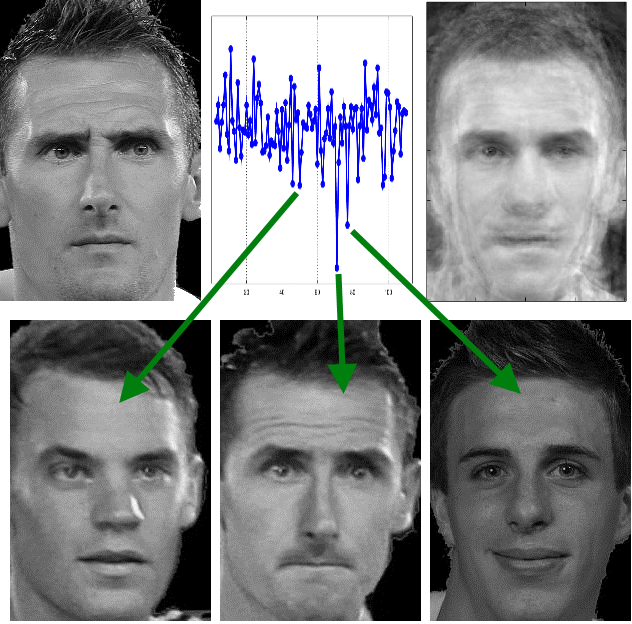
\includegraphics[height=0.93\hsize]{KloseGuess.png} 
\caption{Best approximation of a picture not in the database and guesses based
         on eigenface estimation
        }
\end{figure}

\medskip

% %%%%%%%%%%%%%%%%%%%%%%%%%%%%%%%%%%%%%%%%%%%%%%%%%%%%%%%%%%%%%%%%%%%%%%%%%%%%%%
% REFERNCES %%%%%%%%%%%%%%%%%%%%%%%%%%%%%%%%%%%%%%%%%%%%%%%%%%%%%%%%%%%%%%%%%%%%
% %%%%%%%%%%%%%%%%%%%%%%%%%%%%%%%%%%%%%%%%%%%%%%%%%%%%%%%%%%%%%%%%%%%%%%%%%%%%%%
\sect{References}

\begin{thebibliography}{1}
\bibitem{rule110} \url{https://en.wikipedia.org/wiki/Rule_110}
\bibitem{cca}     \url{https://en.wikipedia.org/wiki/Cyclic_cellular_automaton}
\bibitem{pearson} John Pearson: Complex pattern in a simple system, Science 1993, 189--192
\bibitem{matlabguide} Higham, Higham: Matlab Guide (2nd ed.), SIAM 2005
\bibitem{soma} \url{https://en.wikipedia.org/wiki/Soma_cube}
\bibitem{oct} \url{https://en.wikipedia.org/wiki/Octahedral_symmetry}
\bibitem{manyface} \url{https://de.wikipedia.org/wiki/Liste_der_deutschen_Fu\%C3\%9Fballnationalspieler/*}
\bibitem{face} Muller, Magaia, Herbst: Singular Value Decompostion, Eigenfaces,
               and 3D Reconstructions, SIAM REVIEW (46) 518--545, 2004
\end{thebibliography}

\end{multicols}
\end{frame}
\end{document}
